%doc: Revista 3/La castanyada/ELS CASTANYERS I LES CASTANYERES.docx
\newpage

\begin{news}
{2} %columnes
{Els castanyers i les castanyeres}
{Els nois i noies de 1r d’ESO,  van fer de castanyers i castanyeres als nens i nenes de parvulari i primària}
{ESO}
{216} %pagesof


\noindent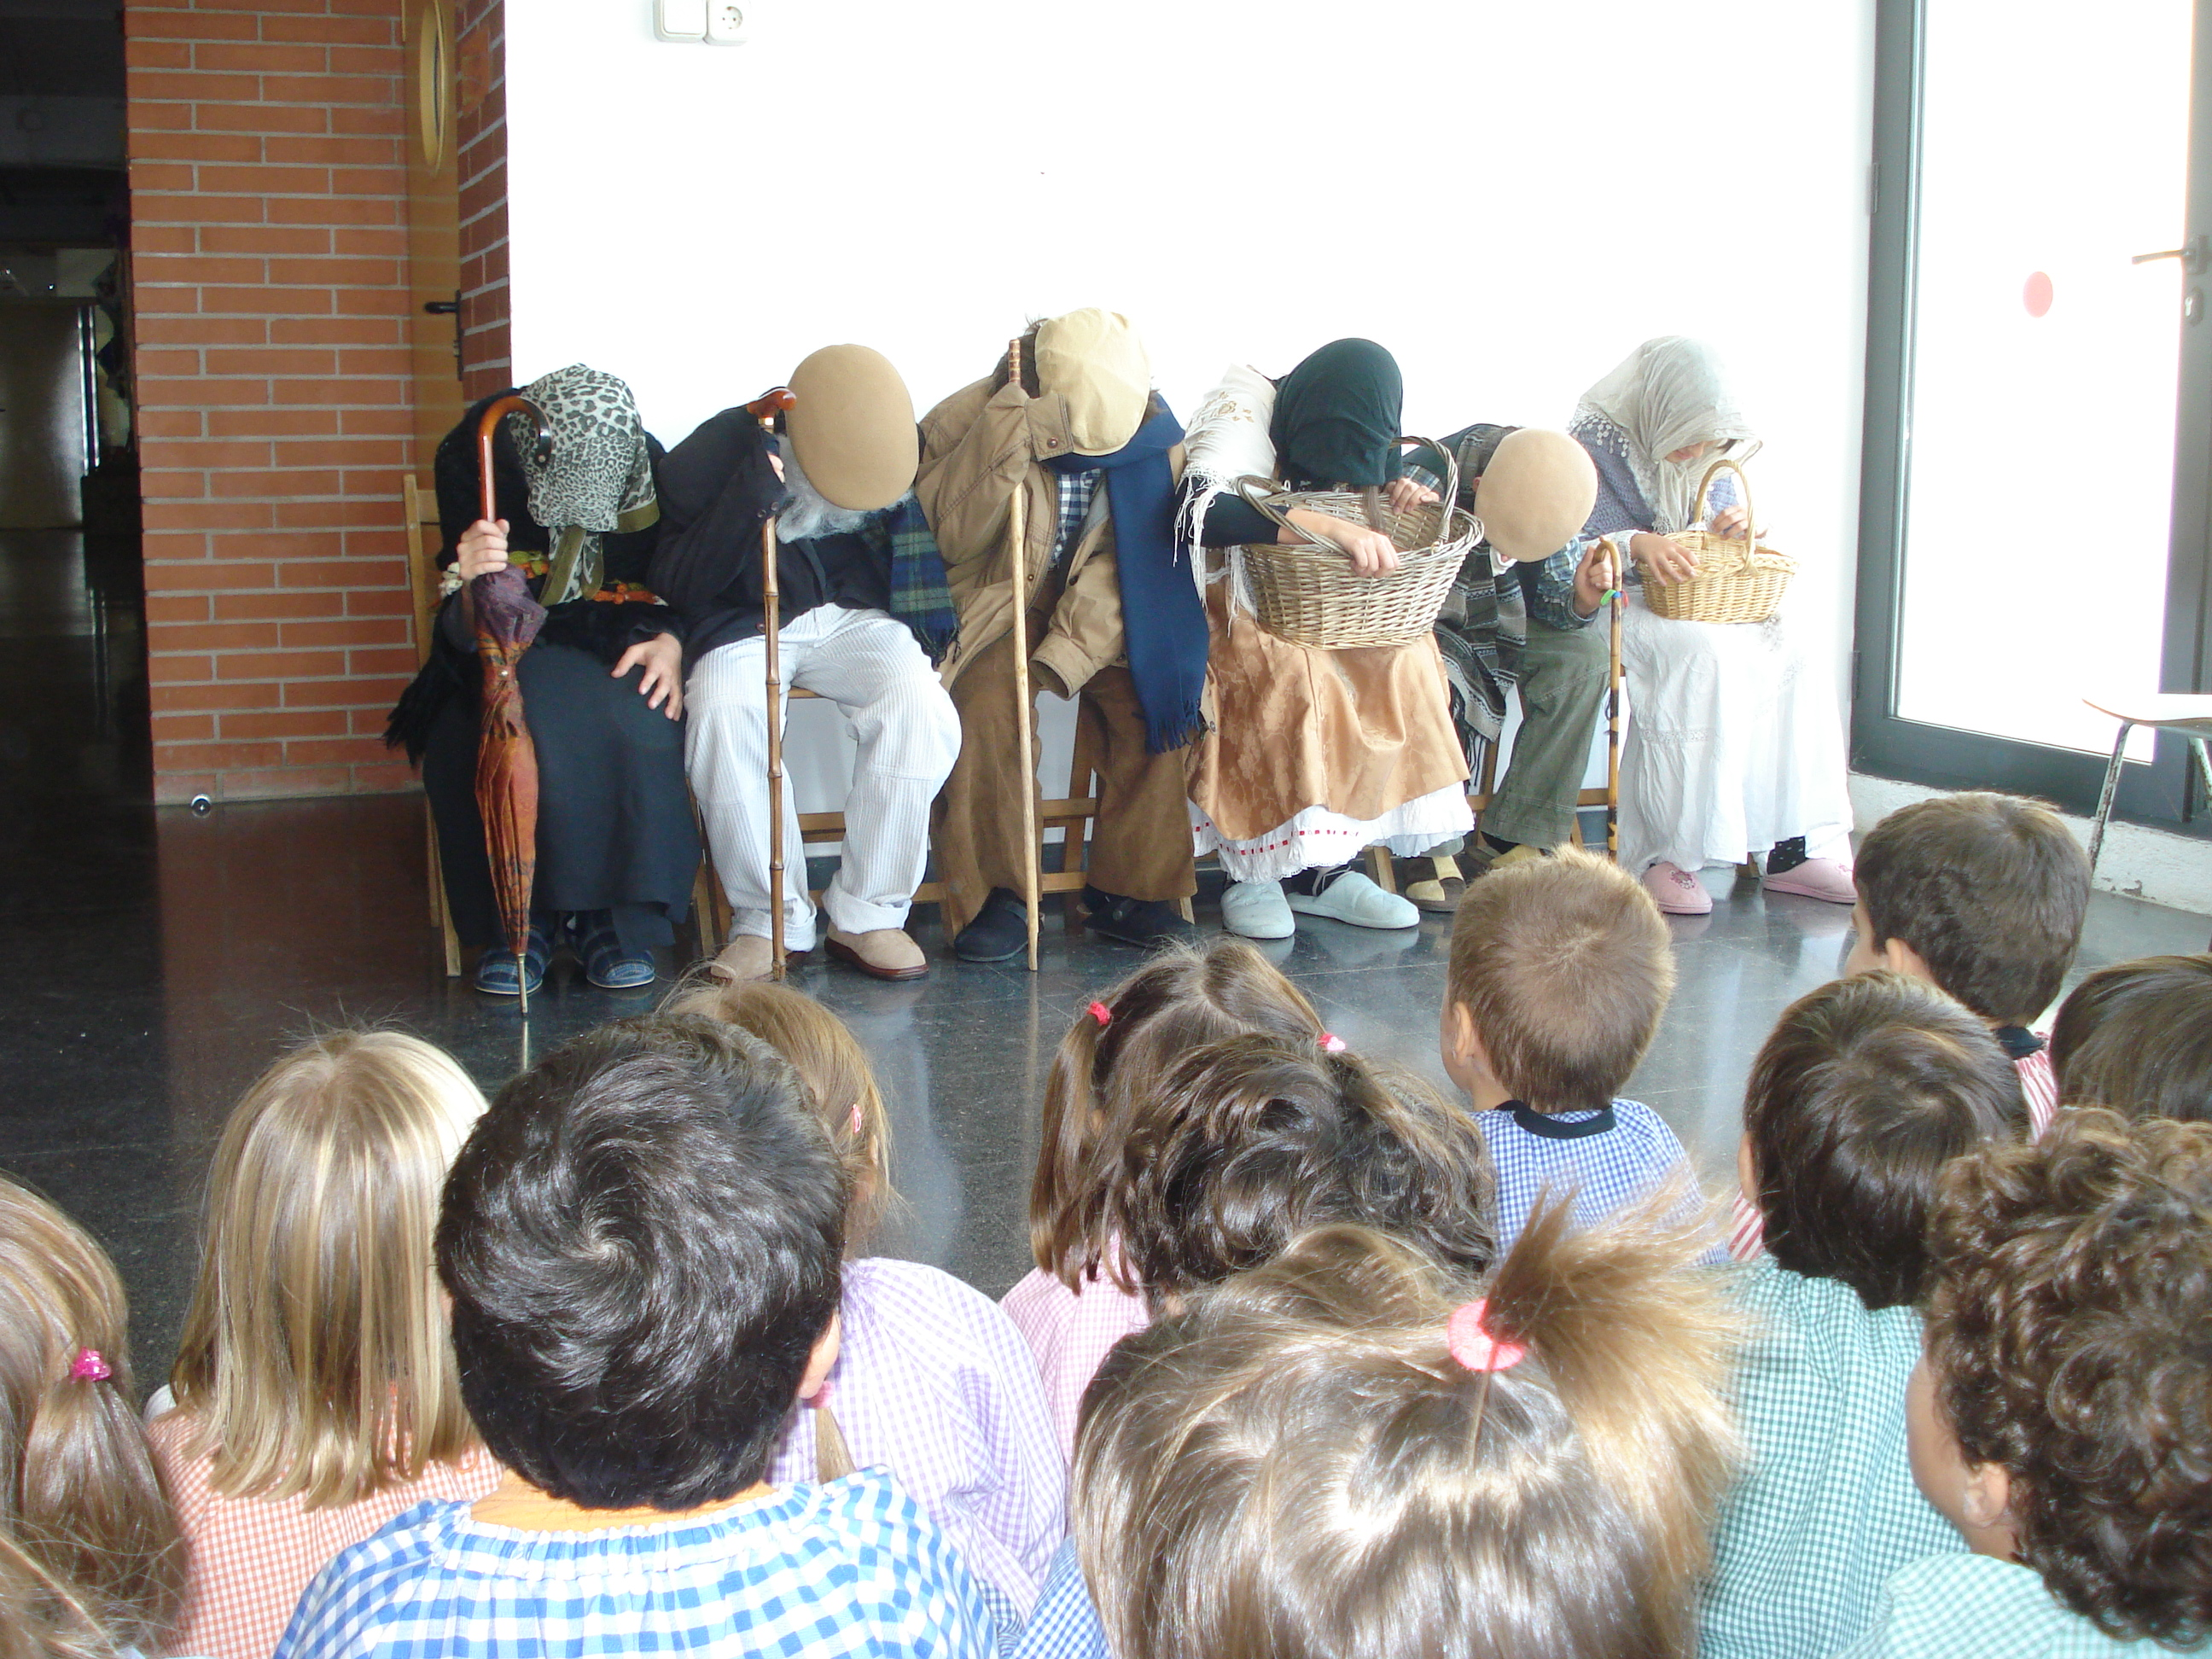
\includegraphics[width=8.5cm,keepaspectratio]{parvulari/img/castanyada_fiotos012.jpg}
El divendres  29 d’octubre,  sis nois i noies de 1r d’ESO,  l’Oriol, la Laia, l’Òscar, el Joel, el Dídac i l’Ariadna,  van anar a fer una representació als nens i nenes de parvulari i primària. Van fer de castanyers i castanyeres. Ho van fer molt bé, tenien moltes ganes de poder-la representar, els feia molta il.lusió.

Els nens i nenes petits es van quedar bocabadats, els va agradar molt, feien una cara de sorpresos, que em sembla que tots s’ho van creure!

El vestuari que portaven estava molt ben trobat; em penso que per a ells no va ser fàcil fer la representació, no només s’havien de disfressar, sinó que també van haver de fer una veu especial, moure els braços i les cames com els vells, i, sobretot, no tenir gens de vergonya! 

A tots els va agradar molt la història que van explicar de la castanya daurada, però també els va agradar moltíssim la cançó que van ballar al final.

Van ser unes castanyeres i castanyers molt valents, simpàtics i gens vergonyosos!!!

\noindent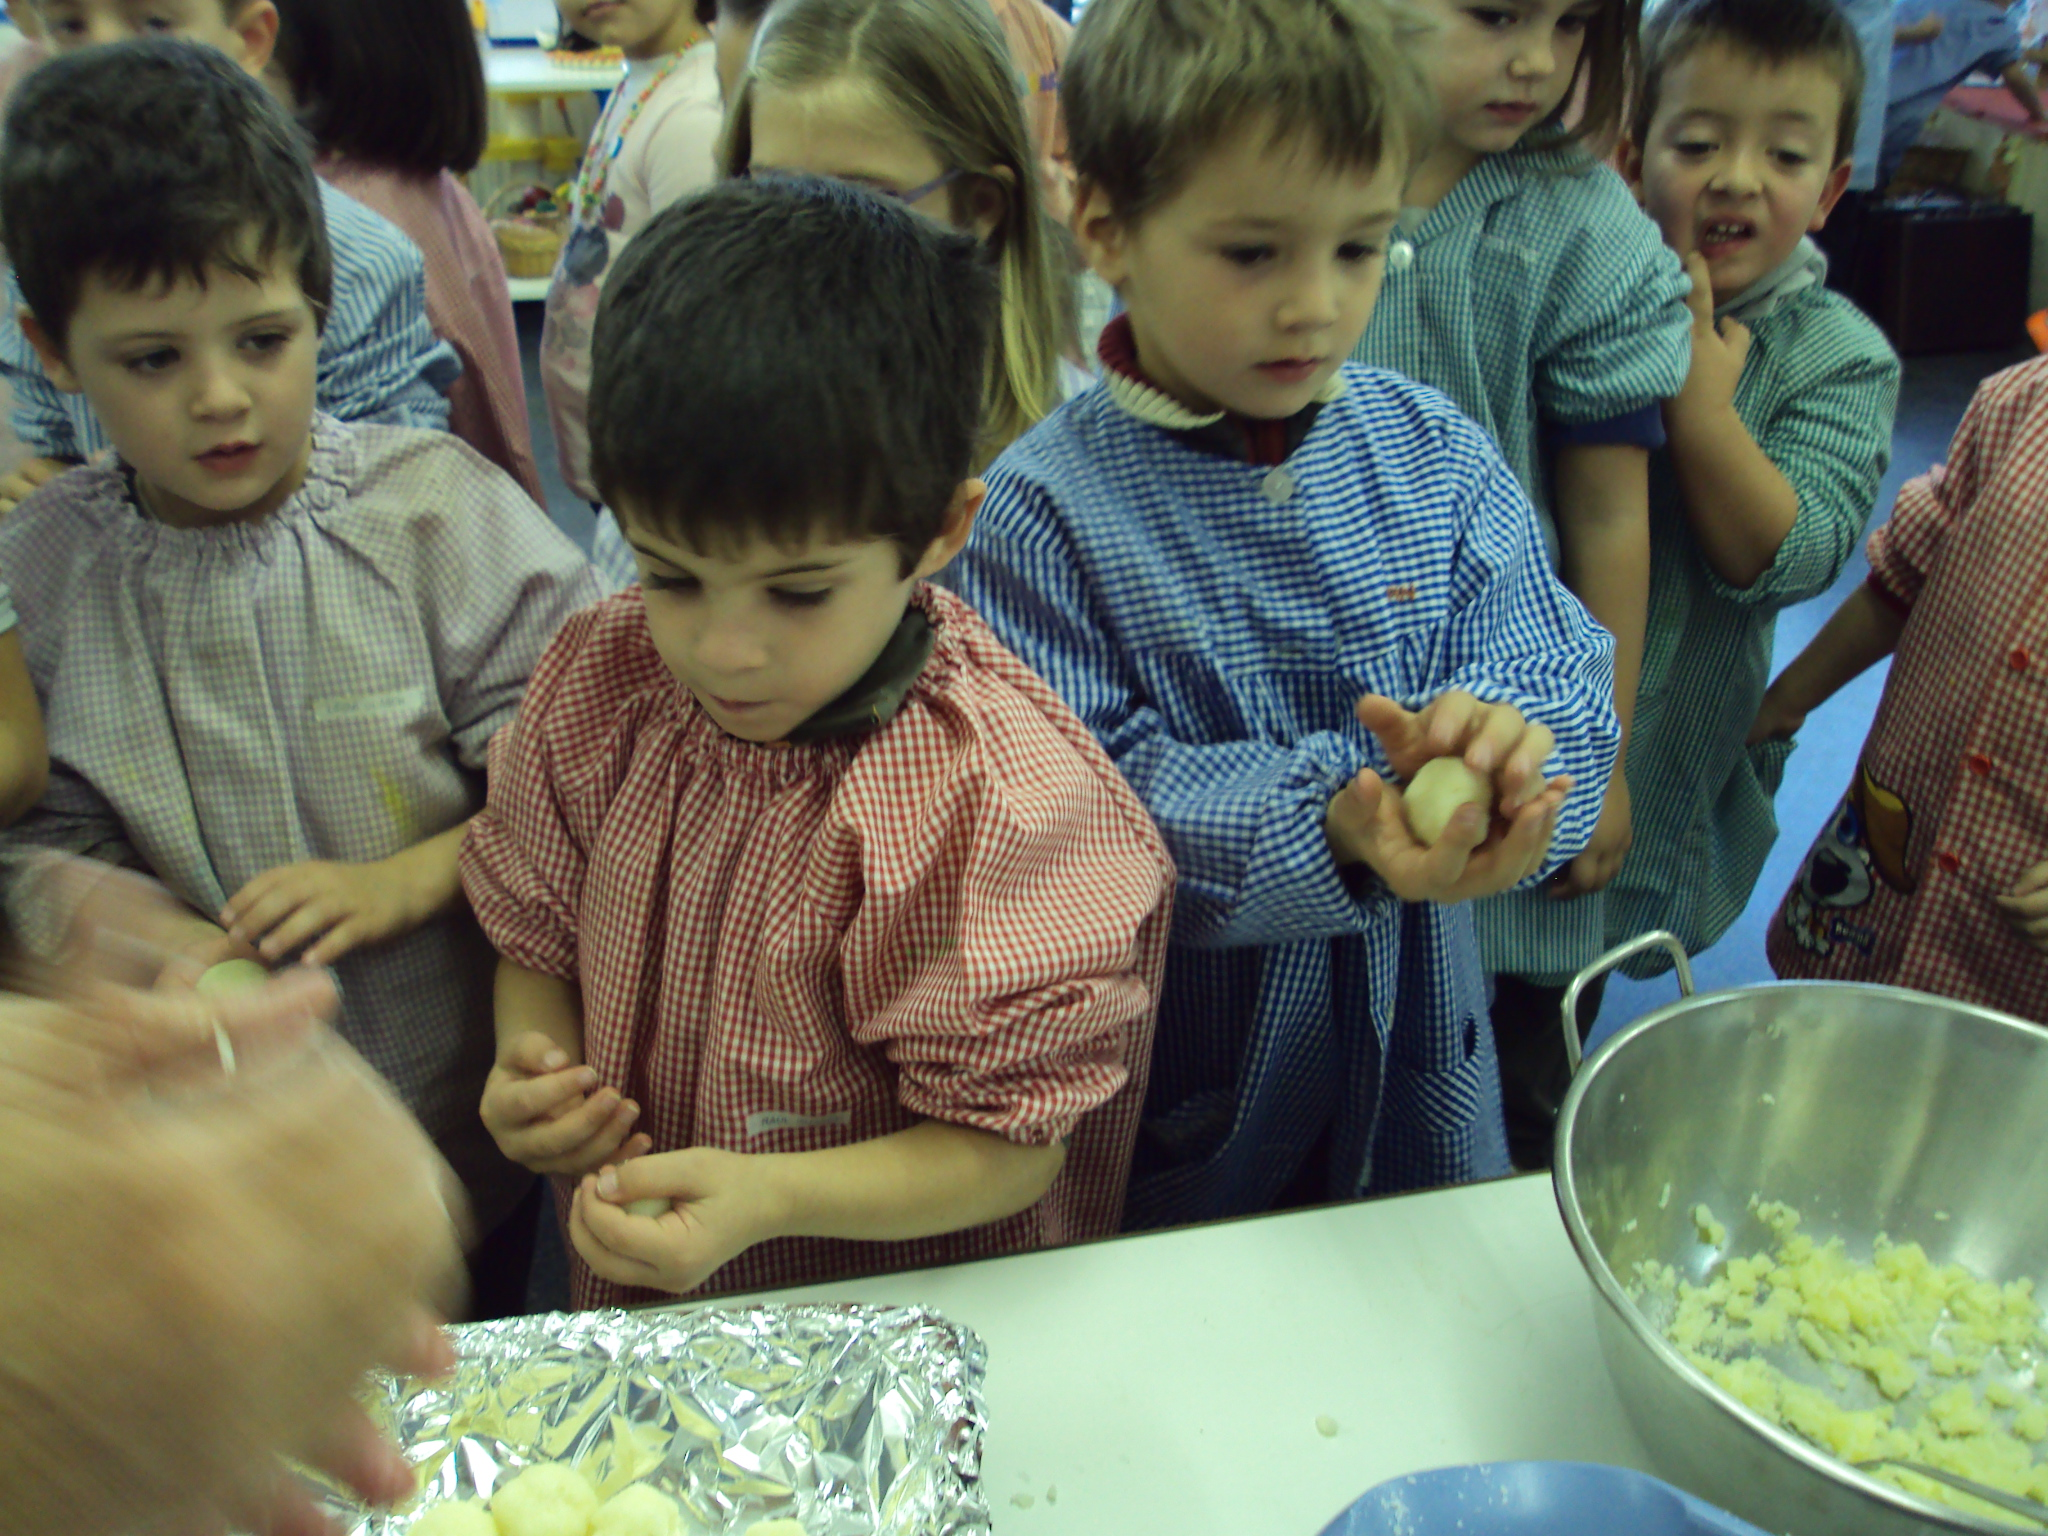
\includegraphics[width=8.5cm,keepaspectratio]{parvulari/img/castanyada_DSC00666.JPG}

\noindent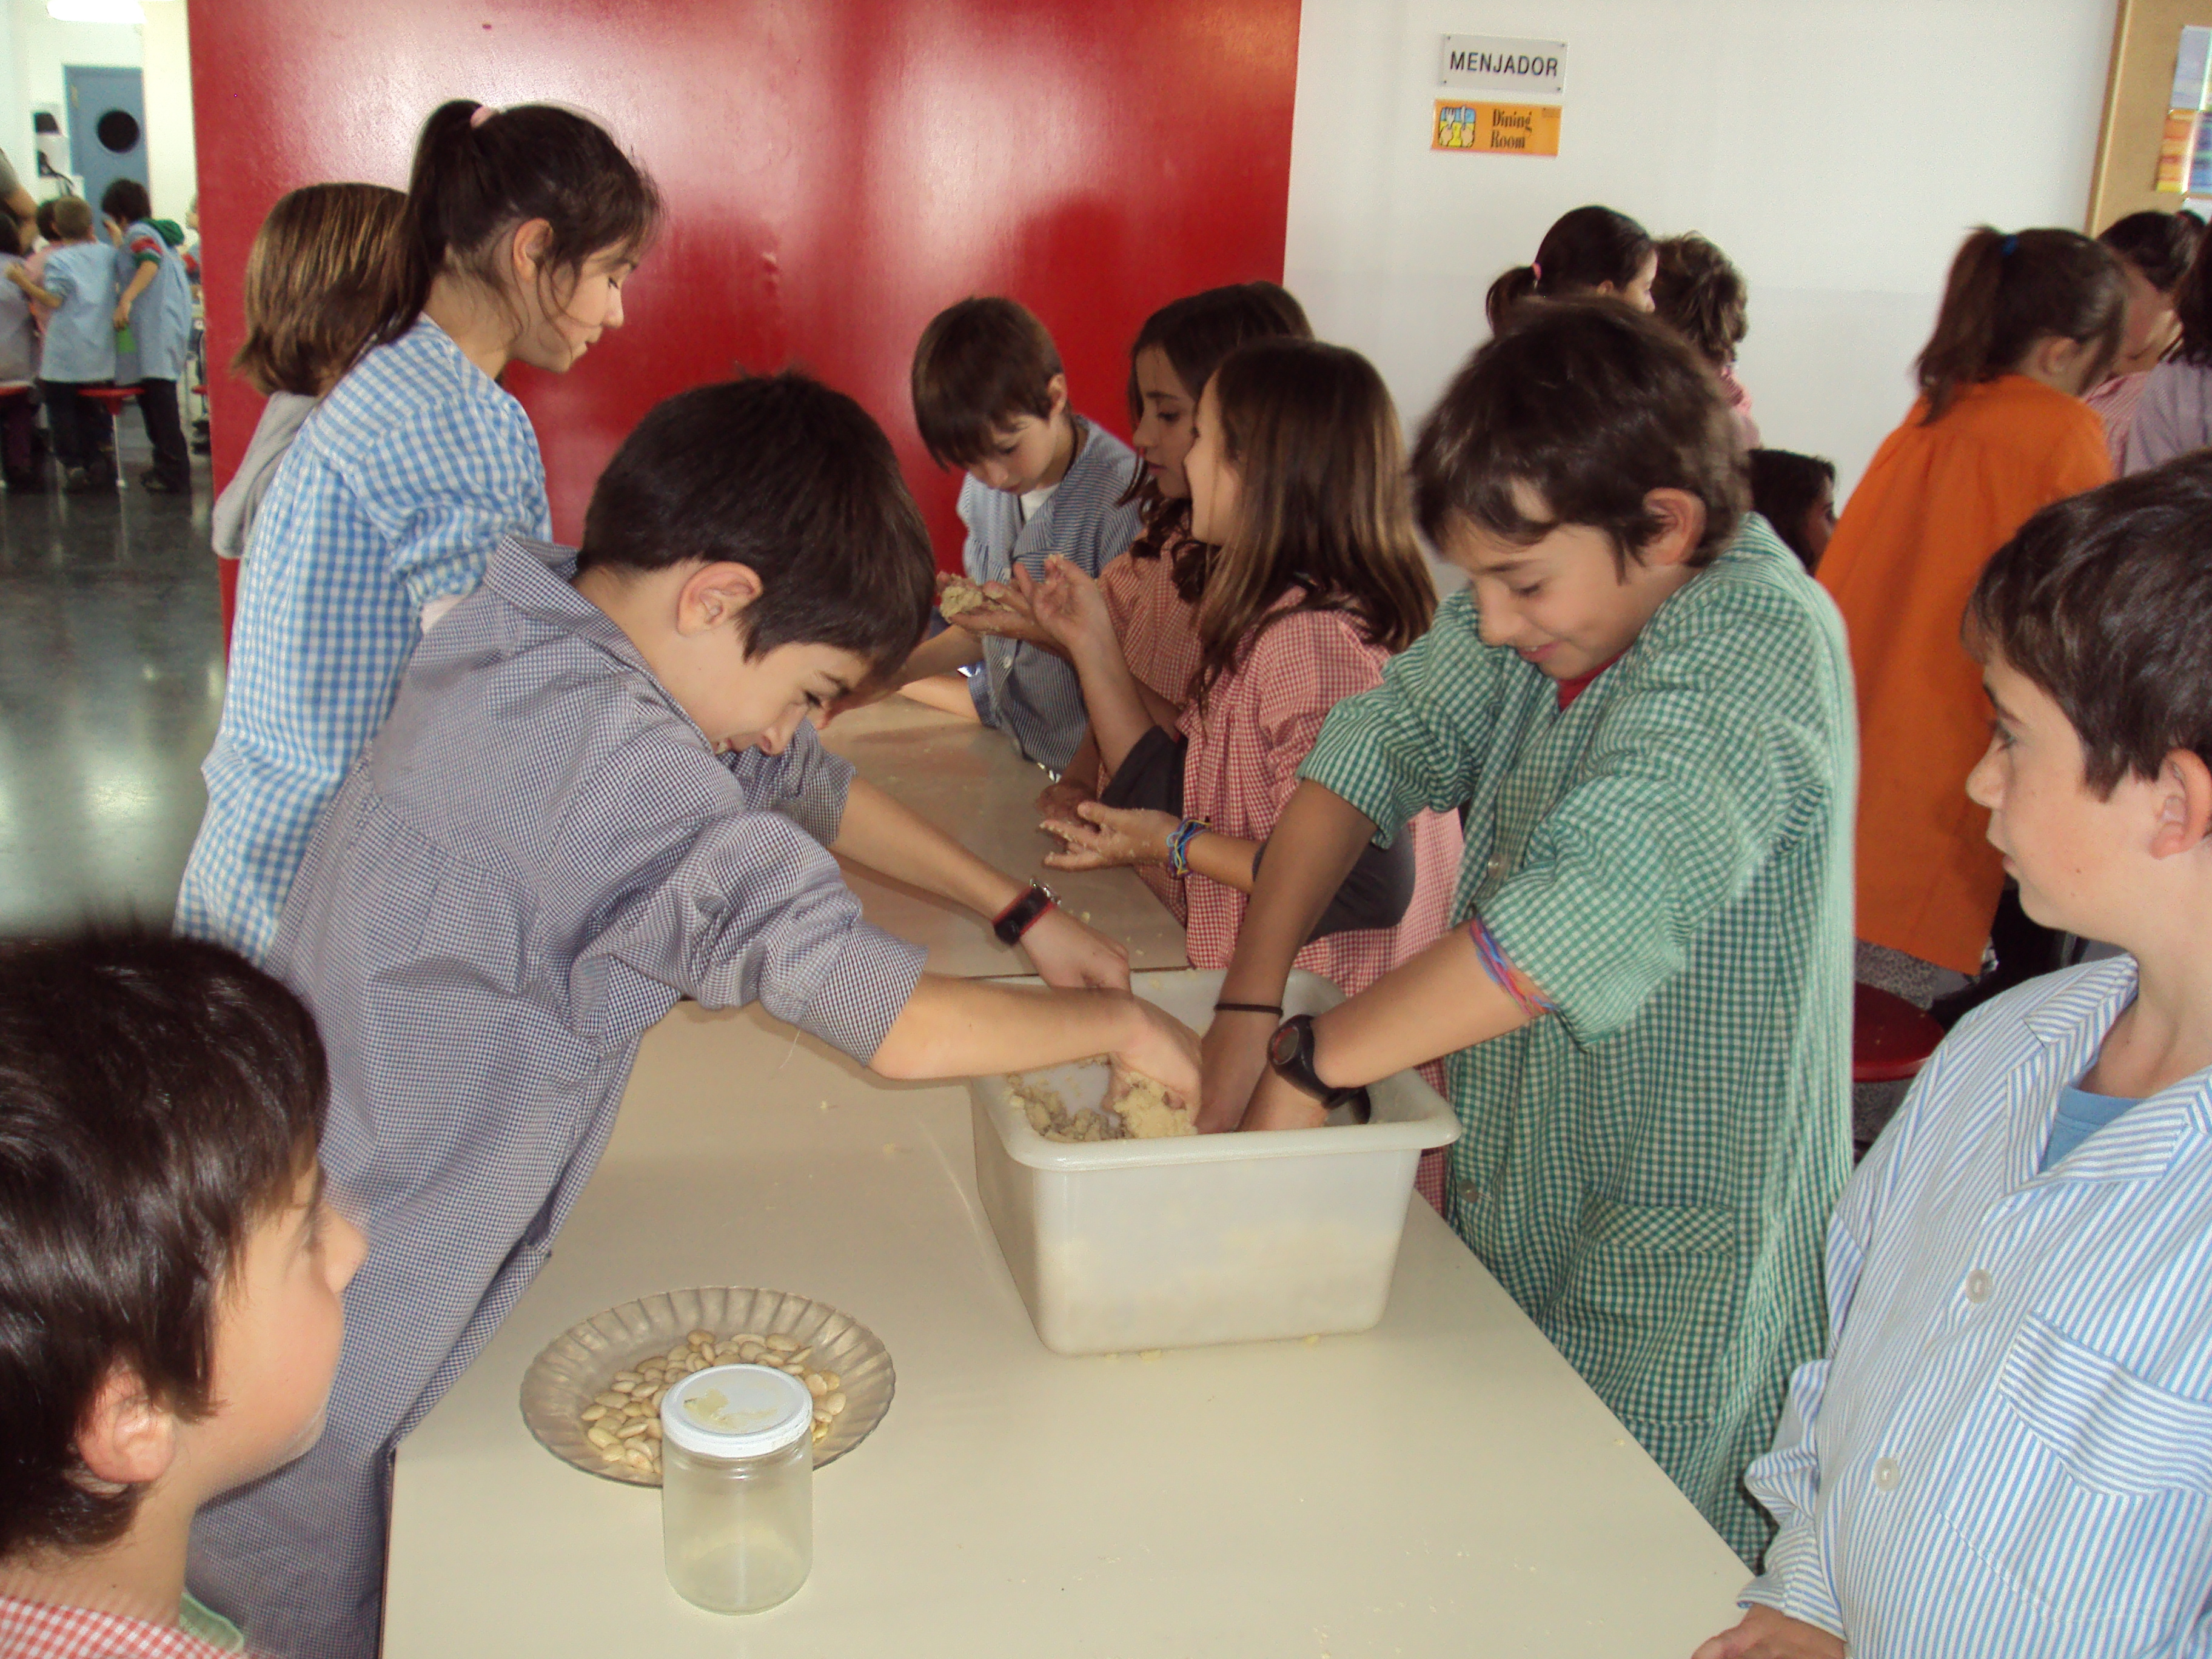
\includegraphics[width=8.5cm,keepaspectratio]{parvulari/img/castanyada_DSC01046.JPG}

\authorandplace{Mariona Medrano}{1r d’ESO}
						
\end{news}
